\documentclass[
	a4paper,
	oneside,
	BCOR = 10mm,
	DIV = 12,
	12pt,
	headings = normal,
]{scrartcl}

%%% Length calculations
\usepackage{calc}
%%%

%%% Support for color
\usepackage{xcolor}
\definecolor{lightblue}{HTML}{03A9F4}
\definecolor{red}{HTML}{F44336}
%%%

%%% Including graphics
\usepackage{graphicx}
%%%

%%% Font selection
\usepackage{fontspec}

\setromanfont{STIX Two Text}[
	SmallCapsFeatures = {LetterSpace = 8},
]

\setsansfont{IBM Plex Sans}[
	Scale = MatchUppercase,
]

\setmonofont{IBM Plex Mono}[
	Scale = MatchUppercase,
]
%%%

%%% Math typesetting
\usepackage{amsmath}

\usepackage{unicode-math}
\setmathfont{STIX Two Math}

\usepackage{IEEEtrantools}
%%%

%%% List settings
\usepackage{enumitem}
\setlist[enumerate]{
	label*      = {\arabic*.},
	leftmargin  = *,
	labelindent = \parindent,
	topsep      = 1\baselineskip,
	parsep      = 0\baselineskip,
	itemsep     = 1\baselineskip,
	noitemsep, % override itemsep
}

\setlist[itemize]{
	label*      = {—},
	leftmargin  = *,
	labelindent = \parindent,
	topsep      = 1\baselineskip,
	parsep      = 0\baselineskip,
	itemsep     = 1\baselineskip,
	noitemsep, % override itemsep
}

\setlist[description]{
	font        = {\rmfamily\upshape\bfseries},
	topsep      = 1\baselineskip,
	parsep      = 0\baselineskip,
	itemsep     = 0\baselineskip,
}

%%%

%%% Structural elements typesetting
\setkomafont{pagenumber}{\rmfamily\upshape}
\setkomafont{disposition}{\rmfamily\bfseries}

% Sectioning
\RedeclareSectionCommand[
	beforeskip = -1\baselineskip,
	afterskip  = 1\baselineskip,
	font       = {\normalsize\bfseries\scshape},
]{section}

\RedeclareSectionCommand[
	beforeskip = -1\baselineskip,
	afterskip  = 1\baselineskip,
	font       = {\normalsize\bfseries\itshape},
]{subsection}

\RedeclareSectionCommand[
	beforeskip = -1\baselineskip,
	afterskip  = 1\baselineskip,
	font       = {\normalsize\bfseries},
]{subsubsection}

\RedeclareSectionCommand[
	beforeskip = -1\baselineskip,
	afterskip  = -0.5em,
	font       = {\normalsize\mdseries\scshape\addfontfeatures{Letters = {UppercaseSmallCaps}}},
]{paragraph}
%%%

%%% Typographic enhancements
\usepackage{microtype}
%%%

%%% Language-specific settings
\usepackage{polyglossia}
\setmainlanguage{ukrainian}
\setotherlanguages{english}
%%%

%%% Captions
\usepackage{caption}
\usepackage{subcaption}

%\DeclareCaptionLabelFormat{closing}{#2)}
%\captionsetup[subtable]{labelformat = closing}

%\captionsetup[subfigure]{labelformat = closing}

\captionsetup[table]{
	aboveskip = 0\baselineskip,
	belowskip = 0\baselineskip,
}

\captionsetup[figure]{
	aboveskip = 1\baselineskip,
	belowskip = 0\baselineskip,
}

\captionsetup[subfigure]{
	labelformat = simple,
	labelformat = brace,
}
%%%

%%% Hyphenated ragged typesetting
\usepackage{ragged2e}
%%%

%%% Table typesetting
\usepackage{booktabs}
\usepackage{longtable}

\usepackage{multirow}

\usepackage{array}
\newcolumntype{v}[1]{>{\RaggedRight\arraybackslash\hspace{0pt}}p{#1}}
\newcolumntype{b}[1]{>{\Centering\arraybackslash\hspace{0pt}}p{#1}}
\newcolumntype{n}[1]{>{\RaggedLeft\arraybackslash\hspace{0pt}}p{#1}}
%%%

%%% Drawing
\usepackage{tikz}
\usepackage{tikzscale}
\usetikzlibrary{positioning}
\usetikzlibrary{arrows.meta} % Stealth arrow tips
\usetikzlibrary{shapes.geometric} % Stealth arrow tips
%%%

%%% SI units typesetting
\usepackage{siunitx}
\sisetup{
	output-decimal-marker = {,},
	exponent-product      = {\cdot},
	inter-unit-product    = \ensuremath{{} \cdot {}},
	per-mode              = symbol,
}
%%%

%%% Framing code listings
\usepackage{tcolorbox}
\tcbuselibrary{breakable}
\tcbuselibrary{minted}
\tcbuselibrary{skins}

\newtcblisting[
	auto counter, 
	list inside, 
	number within = section,
]{listingpython}[3][]{%
	minted language = python,
	minted style    = bw,
	minted options  = {
		linenos,
		tabsize = 4,
		breaklines,
		% breakanywhere,
		fontsize = \footnotesize,
		autogobble
	},
	%
	% empty,
	sharp corners,
	colframe         = black,
	colback          = black!0,
	leftrule         = 0em,
	rightrule        = 0em,
	toprule          = 1pt, % orig = 0pt
	bottomrule       = 1pt, % orig = 0pt
	titlerule        = 0.5pt,
	colbacktitle     = black!0,
	coltitle         = black,
	toptitle         = 0.3em,
	bottomtitle      = 0.1em,
	borderline north = {1pt}{0pt}{black},
	borderline south = {1pt}{0pt}{black},
	before skip      = \intextsep,
	after  skip      = \intextsep,
	title            = {Лістинг \thetcbcounter: #2},
	list entry       = {\protect\numberline{\thetcbcounter}#2},
	left = 0em,
	right = 0em,
	%
	listing only,
	breakable,
	%
	label = {#3},
	%
	#1
}

\newtcbinputlisting[auto counter, list inside, number within = section]{\inputpython}[4][]{%
	minted language = python,
	minted style    = bw,
	minted options  = {
		linenos,
		tabsize = 4,
		breaklines,
		breakbytokenanywhere,
		fontsize = \footnotesize,
	},
	%
	% empty,
	sharp corners,
	colframe         = black,
	colback          = black!0,
	leftrule         = 0em,
	rightrule        = 0em,
	toprule          = 0pt, % orig = 0pt
	bottomrule       = 0pt, % orig = 0pt
	titlerule        = 0.5pt,
	colbacktitle     = black!0,
	coltitle         = black,
	toptitle         = 0.3em,
	bottomtitle      = 0.1em,
	borderline north = {1pt}{0pt}{black},
	borderline south = {1pt}{0pt}{black},
	before skip      = \intextsep,
	after  skip      = \intextsep,
	title            = {Лістинг \thetcbcounter: #3},
	list entry       = {\protect\numberline{\thetcbcounter}#3},
	left = 0em,
	right = 0em,
	%
	listing file={#2},
	listing only,
	breakable,
	%
	label = {#4},
	%
	#1
}

% Customize minted
\usepackage{minted}
\setmintedinline{
	style = bw,
	breaklines,
}

% Customize minted line numbers
\renewcommand{\theFancyVerbLine}{\ttfamily\scriptsize\arabic{FancyVerbLine}}

%%%

%%% Custom Q & A environments
\ExplSyntaxOn
    \NewDocumentEnvironment{question} { o }
     {
      \par\noindent
      \IfNoValueTF{#1} { \textsc{Запитання:~} }{ \textsc{Запитання~#1:~} }
       \ignorespaces
     }
     {}
\ExplSyntaxOff
%%%

%%% Links and hyperreferences
\usepackage{hyperref}
\hypersetup{
	bookmarksnumbered = true,
	colorlinks      = false,
	linkbordercolor = red,
	urlbordercolor  = lightblue,
	pdfborderstyle  = {/S/U/W 1.5},
}
%%%

%%% Length adjustments
% Set baselineskip, default is 14.5 pt
\linespread{1.068966} % ~15.5 pt
\setlength{\emergencystretch}{1em}
\setlength{\parindent}{1.5em}
\newlength{\gridunitwidth}
\setlength{\gridunitwidth}{\textwidth / 12}
%%%

%%% Custom commands
\newcommand{\allcaps}[1]{{\addfontfeatures{LetterSpace = 8, Kerning = Off}#1}}
\newcommand{\filename}[1]{\texttt{#1}}
\newcommand{\progname}[1]{\texttt{#1}}
\newcommand{\modulename}[1]{\texttt{#1}}
%%%

%%% Custom math commands
\newcommand{\longvar}[1]{\mathit{#1}}
%%%

\begin{document}

\begin{titlepage}
		\begin{center}
			Міністерство освіти і науки України\\
			Національний авіаційний університет\\
			Навчально-науковий інститут комп'ютерних інформаційних технологій\\
			Кафедра комп'ютеризованих систем управління

			\vspace{\fill}
				Лабораторна робота №2\\
				з~дисципліни «Комп'ютерні системи»\\
				на~тему «Моделювання часових характеристик обчислювальних систем та~мереж»\\
				Варіант~№3

			\vspace{\fill}

			\begin{flushright}
				Виконав:\\
				студент \allcaps{ННІКІТ}\\
				групи СП-325\\
				Клокун В.\,Д.\\
				Перевірив:\\
				Ковальов М.\,О.
			\end{flushright}

			Київ 2019
		\end{center}
	\end{titlepage}

	\section{Мета роботи}
		Вивчення методів оцінки трудомісткості алгоритмів.

	\section{Хід роботи}
		Вихідними даними для лабораторної роботи є схема алгоритму~(рис.~\ref{fig:flowchart}). 

		\begin{figure}[!htbp]
			\centering
			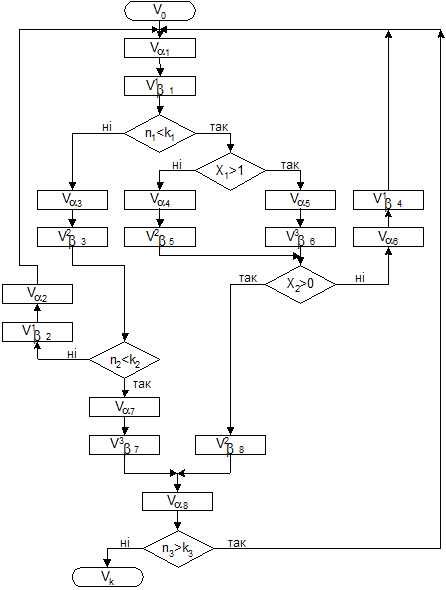
\includegraphics[height = 30\baselineskip]{./assets/y03s02-compsys-lab-02-p01.png}
			\caption{Схема алгоритму}
			\label{fig:flowchart}
		\end{figure}

		\subsection{Обчислення середньої кількості операцій за один прогін алгоритму}
			Нехай~$n_1, \dots, n_{k-1}$~— середня кількість звернень до~операторів~$v_1, \dots, v_{k - 1}$. Тоді середня кількість операцій за один прогін алгоритму~$\theta_{\text{осн}}$ визначається так:
			\begin{IEEEeqnarray}{rCl}
				\label{eq:avg-op-cnt-per-run}
				\theta_{\text{осн}} = \sum_{} n_i \cdot k_i.
			\end{IEEEeqnarray}
			Щоб знайти значення середньої кількості звернень~$n_1, \dots, n_{k-1}$, за~схемою алгоритму визначаємо та~будуємо матрицю ймовірностей переходу, в~якій кожен елемент~$P_{ij}$ визначає ймовірність переходу із стану~$i$ в~стан~$j$~(табл.~\ref{tab:transition-prob}). 

			\begin{table}[!htbp]
				\centering
				\caption{Матриця ймовірностей переходу схеми алгоритму}
				\label{tab:transition-prob}
				\begin{tabular}{
					l
					*{9}{r}
				}
					\toprule
						& $V_{\alpha{}1}$ & $V_{\alpha{}2}$ & $V_{\alpha{}3}$ & $V_{\alpha{}4}$ & $V_{\alpha{}5}$ & $V_{\alpha{}6}$ & $V_{\alpha{}7}$ & $V_{\alpha{}8}$ & $V_{k}$ \\ 
					\midrule
						$V_{\alpha{}1}$ & & & \num{0.9} & \num{0.025} & \num{0.075}\\
						$V_{\alpha{}2}$ & \num{1} \\
						$V_{\alpha{}3}$ & & \num{0.95} & & & & & \num{0.05} \\
						$V_{\alpha{}4}$ & & & & & & \num{0.75} & & \num{0.25}\\
						$V_{\alpha{}5}$ & & & & & & \num{0.75} & & \num{0.25}\\
						$V_{\alpha{}6}$ & \num{1} \\
						$V_{\alpha{}7}$ & & & & & & & & \num{1} & \\
						$V_{\alpha{}8}$ & \num{0.03} & & & & & & & & \num{0.97} \\
					\bottomrule
				\end{tabular}
			\end{table}

			За матрицею ймовірностей переходу складаємо систему лінійних алгебраїчних рівнянь:
			\begin{IEEEeqnarray}{c}
				\label{eq:sys}
				\left\{ \,
				\begin{IEEEeqnarraybox}[][c]{rCrCrCrCrCrCrCrCrCrCl}
					\IEEEstrut
					-n_1 &+& n_2 &&  &&  &&  &+& n_6 &&  &+& \num{0.03} n_8 &=& -1,\\
								 && -n_2 &+& \num{0.95}n_3 &&  &&  &&  &&  &&  &=& 0,\\
					\num{0.9} n_1 && &&  -n_3 &&  &&  &&  &&  &&  &=& 0,\\
					\num{0.025} n_1 &&    &&  &&  -n_4 &&  &&  &&  &&  &=& 0,\\
					\num{0.075} n_1 &&    &&  &&  &&  -n_5 &&  &&  &&  &=& 0,\\
					 &&    &&  && \num{0.75} n_4 &+& \num{0.75} n_5 &&  -n_6 &&  &&  &=& 0,\\
					 &&    && \num{0.05}n_3 &&  &&  &&  &&  -n_7 &&  &=& 0,\\
					 &&    &&  && \num{0.25}n_4 &+& \num{0.25}n_5 &&  &+& n_7 && -n_8 &=& 0.
					% P_{1(k-1)} n_{1} &+& P_{2(k-1)} n_{2}   &+& \dots &+& (P_{(k-1)(k-1)} – 1) n_{k-1} &=& 0.
					\IEEEstrut
				\end{IEEEeqnarraybox}
				\right.
			\end{IEEEeqnarray}
			Знаходимо розв'язок системи лінійних алгебраїчних рівнянь і записуємо його:
			\begin{IEEEeqnarray*}{rCl'rCl'rCl'rCl}
				n_1 &=& \frac{10000}{679} , &% \approx \num{14.73}
				n_2 &=& \frac{ 8550}{679} , &% \approx \num{12.59}
				n_3 &=& \frac{ 9000}{679} , &% \approx \num{13.25}
				n_4 &=& \frac{  250}{679} , \\[2\jot] % \approx \num{ 0.39}
				n_5 &=& \frac{  750}{679} , &% \approx \num{ 1.10}
				n_6 &=& \frac{  750}{679} , &% \approx \num{ 1.10}
				n_7 &=& \frac{  450}{679} , &% \approx \num{ 0.66}
				n_8 &=& \frac{  700}{679} .  % \approx \num{ 1.03}
			\end{IEEEeqnarray*}
			Отже, розв'язавши систему рівнянь, отримали середні кількості звернень~$n_{1}, \dots, n_{k-1}$ до~операторів~$V_{1}, \dots, V_{k-1}$. 

			Щоб обчислити значення середньої кількості операцій за один прогін алгоритму~$\theta_{\text{осн}}$, необхідно знати значення кількості операцій~$k_i$ кожного оператора~$V_{\alpha{}i}$~(для~заданого варіанту~№3~— табл.~\ref{tab:ki-vals}). 

			\begin{table}[!htbp]
				\centering
				\caption{Число операцій~$k_i$, що складають оператор~$V_{\alpha{}i}$}
				\label{tab:ki-vals}
				\begin{tabular}{
					v{4\gridunitwidth - 2\tabcolsep}
					*{8}{n{1\gridunitwidth - 2\tabcolsep}}
				}
					\toprule
						Номер варіанта & \multicolumn{8}{r}{Кількість операторів~$V_{\alpha}$} \\
						\cmidrule(lr){2-9}
						 & $V_{\alpha{}_1}$ & $V_{\alpha{}_2}$ & $V_{\alpha{}_3}$ & $V_{\alpha{}_4}$ & $V_{\alpha{}_5}$ & $V_{\alpha{}_6}$ & $V_{\alpha{}_7}$ & $V_{\alpha{}_8}$ \\ 
					\midrule
						3 & 30 & 10 & 30 & 20 & 20 & 30 & 50 & 100\\
					\bottomrule
				\end{tabular}
			\end{table}

			Тепер обчислюємо середню кількість операцій за~один прогін алгоритму. Для цього підставляємо задані значення кількості операцій кожного оператора~(табл.~\ref{tab:ki-vals}) у~формулу~\eqref{eq:avg-op-cnt-per-run}:
			\begin{IEEEeqnarray*}{rCl}
				\theta_{\text{осн}} &=& \frac{10000}{679} \cdot 30 + \frac{8550}{679} \cdot 10 + \frac{9000}{679} \cdot 30 + \frac{250}{679} \cdot 20 \\[2\jot] 
														&& \> + \frac{750}{679} \cdot 20 + \frac{750}{679} \cdot 30 + \frac{450}{679} \cdot 50 + \frac{700}{679} \cdot 100\\[2\jot]
														&\approx& \num{1164.21}.
			\end{IEEEeqnarray*}
			Отже, середня кількість операцій за один прогін заданого алгоритму~$\theta_{\text{осн}} \approx \num{1164.21}$. 

		\subsection{Обчислення середньої кількості звернень до~кожного з~файлів}
			Середня кількість звернень до~файлів визначається так:
			\begin{IEEEeqnarray}{rCl}
				N_{h} = \sum_{v_i \in S_{h}} n_i,
			\end{IEEEeqnarray}
			де~$n_i$~— середня кількість звернення до~оператора~$v_i$.

			На~схемі алгоритму вершини з~операціями звернення до~файлів позначені~$V_{\beta{}i}$. Оскільки всі вершини мають різні індекси, вважаємо, що~в~кожній з~них відбувається звернення до~окремого файлу. Також на~схемі алгоритму оператори звернення до~файлів йдуть одразу~ж після основних операторів, отже середня кількість звернення до~операторів звернення до~файлів буде дорівнювати середній кількості звернення до~відповідного основного оператора. Тоді: 
			\begin{IEEEeqnarray*}{rClCl'rClCl'rClCl'rClCl}
				N_{1} &=& n_1 &=& \frac{10000}{679} , &% \approx \num{14.73}
				N_{2} &=& n_2 &=& \frac{ 8550}{679} , &% \approx \num{12.59}
				N_{3} &=& n_3 &=& \frac{ 9000}{679} , &% \approx \num{13.25}
				N_{4} &=& n_4 &=& \frac{  250}{679} , \\[2\jot] % \approx \num{ 0.39}
				N_{5} &=& n_5 &=& \frac{  750}{679} , &% \approx \num{ 1.10}
				N_{6} &=& n_6 &=& \frac{  750}{679} , &% \approx \num{ 1.10}
				N_{7} &=& n_7 &=& \frac{  450}{679} , &% \approx \num{ 0.66}
				N_{8} &=& n_8 &=& \frac{  700}{679} .  % \approx \num{ 1.03}
			\end{IEEEeqnarray*}

			Отже, були знайдені значення середньої кількості звернень до~кожного з~файлів. 

		\subsection{Обчислення середньої кількості інформації, яка~передається при~одному зверненні до~файлу}
			Середня кількість інформації, яка передається при одному зверненні до файлу визначається так:
			\begin{IEEEeqnarray}{rCl}
			\label{eq:avg-data-amount-per-file}
				\theta_{h} = \frac{1}{N_{h}} \sum_{v_{i} \in S_{h}} n_i \cdot l_i, 
			\end{IEEEeqnarray}
			де~$N_{h}$~— середня кількість звернення до~файлу~$F_{h}$, $n_i$~— середня кількість звернення до~оператора~$v_i$, $l_i$~— середня кількість інформації, що~передається при виконанні оператора звернення~$v_{i}$~(табл.~\ref{tab:avg-data-amount}). 

			\begin{table}[!htbp]
				\newlength{\tabtmpgridunit}
				\setlength{\tabtmpgridunit}{9\gridunitwidth / 8}
				%
				\centering
				\caption{Середня кількість інформації~$l_i$, що~передається при~виконанні оператора звернення~$v_{\beta{}i}$}
				\label{tab:avg-data-amount}
				\begin{tabular}{
					v{3\gridunitwidth - 2\tabcolsep}
					*{8}{n{1\tabtmpgridunit - 2\tabcolsep}}
				}
					\toprule
						Номер варіанта & \multicolumn{8}{r}{Кількість інформації}\\
						\cmidrule(lr){2-9}
						 & $V_{\beta{}_1}$ & $V_{\beta{}_2}$ & $V_{\beta{}_3}$ & $V_{\beta{}_4}$ & $V_{\beta{}_5}$ & $V_{\beta{}_6}$ & $V_{\beta{}_7}$ & $V_{\beta{}_8}$ \\ 
					\midrule
						3 & 250 & 500 & 150 & 1000 & 200 & 100 & 400 & 200\\
					\bottomrule
				\end{tabular}
			\end{table}

			Оскільки звернення до кожного з файлів відбувається лише в одній вершині~$N_{h} = n_{h}$. Підставляємо вихідні дані у формулу~\eqref{eq:avg-data-amount-per-file}:
			\begin{IEEEeqnarray*}{rCl'rCl}
				% \theta_{h} &=& \frac{1}{N_{h}} \sum_{v_{i} \in S_{h}} n_i \cdot l_i\\[2\jot]
				\theta_{1} &=& \frac{679}{10000} \cdot \frac{10000}{679} \cdot 250 = \num{250}, &
				\theta_{2} &=& \frac{679}{8550} \cdot \frac{8550}{679} \cdot 500 = \num{500}, \\[2\jot]
				\theta_{3} &=& \frac{679}{9000} \cdot \frac{9000}{679} \cdot 150 = \num{150}, &
				\theta_{4} &=& \frac{679}{250} \cdot \frac{250}{679} \cdot 1000 = \num{1000}, \\[2\jot] 
				\theta_{5} &=& \frac{679}{750} \cdot \frac{750}{679} \cdot 200 = \num{200}, &
				\theta_{6} &=& \frac{679}{750} \cdot \frac{750}{679} \cdot 100 = \num{100}, \\[2\jot]
				\theta_{7} &=& \frac{679}{450} \cdot \frac{450}{679} \cdot 400 = \num{400}, &
				\theta_{8} &=& \frac{679}{700} \cdot \frac{700}{679} \cdot 200 = \num{200}. 
														% &\approx& \num{13136.97}.
			\end{IEEEeqnarray*}
			Отже, знайшли середню кількість інформації, яка~передається при~одному зверненні до~файлу~$\theta_{h}$ для~кожного з~файлів~$F_{h}$. 

		\subsection{Обчислення середньої трудомісткості етапу рахування}
			Середня трудомісткість етапу рахування~$\theta_{\text{О}}$ визначається так:
			\begin{IEEEeqnarray}{c}
			\label{eq:theta-o}
				\theta_{\text{О}} = \frac{\theta}{N},
			\end{IEEEeqnarray}
			де~$N$~— сума середнього числа~$N_{i}$ звернень до~основних операторів~$S_{\text{О}}$, тобто:
			\begin{IEEEeqnarray}{c}
				N = \sum_{i = 1}^{V_{\text{О}i}} n_i,
			\end{IEEEeqnarray}

			Отже, спочатку обчислюємо суму середнього числа звернень до основних операторів~$N$:
			\begin{IEEEeqnarray*}{rCl}
				N = \frac{10000 + 8550 + 9000 + 250 + 750 + 750 + 450 + 700}{679} = \frac{30450}{679} \approx \num{48.85}.
			\end{IEEEeqnarray*}
			Підставляємо отримане значення у~формулу~\eqref{eq:theta-o} і~знаходимо середню трудоміскістість етапу рахування:
			\begin{IEEEeqnarray*}{rCl}
				\theta_{\text{О}} = \frac{790500}{679} \cdot \frac{679}{30450} = \frac{790500}{30450} \approx \num{25.96}.
			\end{IEEEeqnarray*}
			Отже, знайшли значення середньої трудомісткості етапу рахування~$\theta_{\text{О}} = \num{25.96}$.

	\section{Висновок}
		Виконуючи дану лабораторну роботу, ми~вивчили методі оцінки трудомісткості алгоритмів. 

\end{document}

